\begin{figure}
\centering
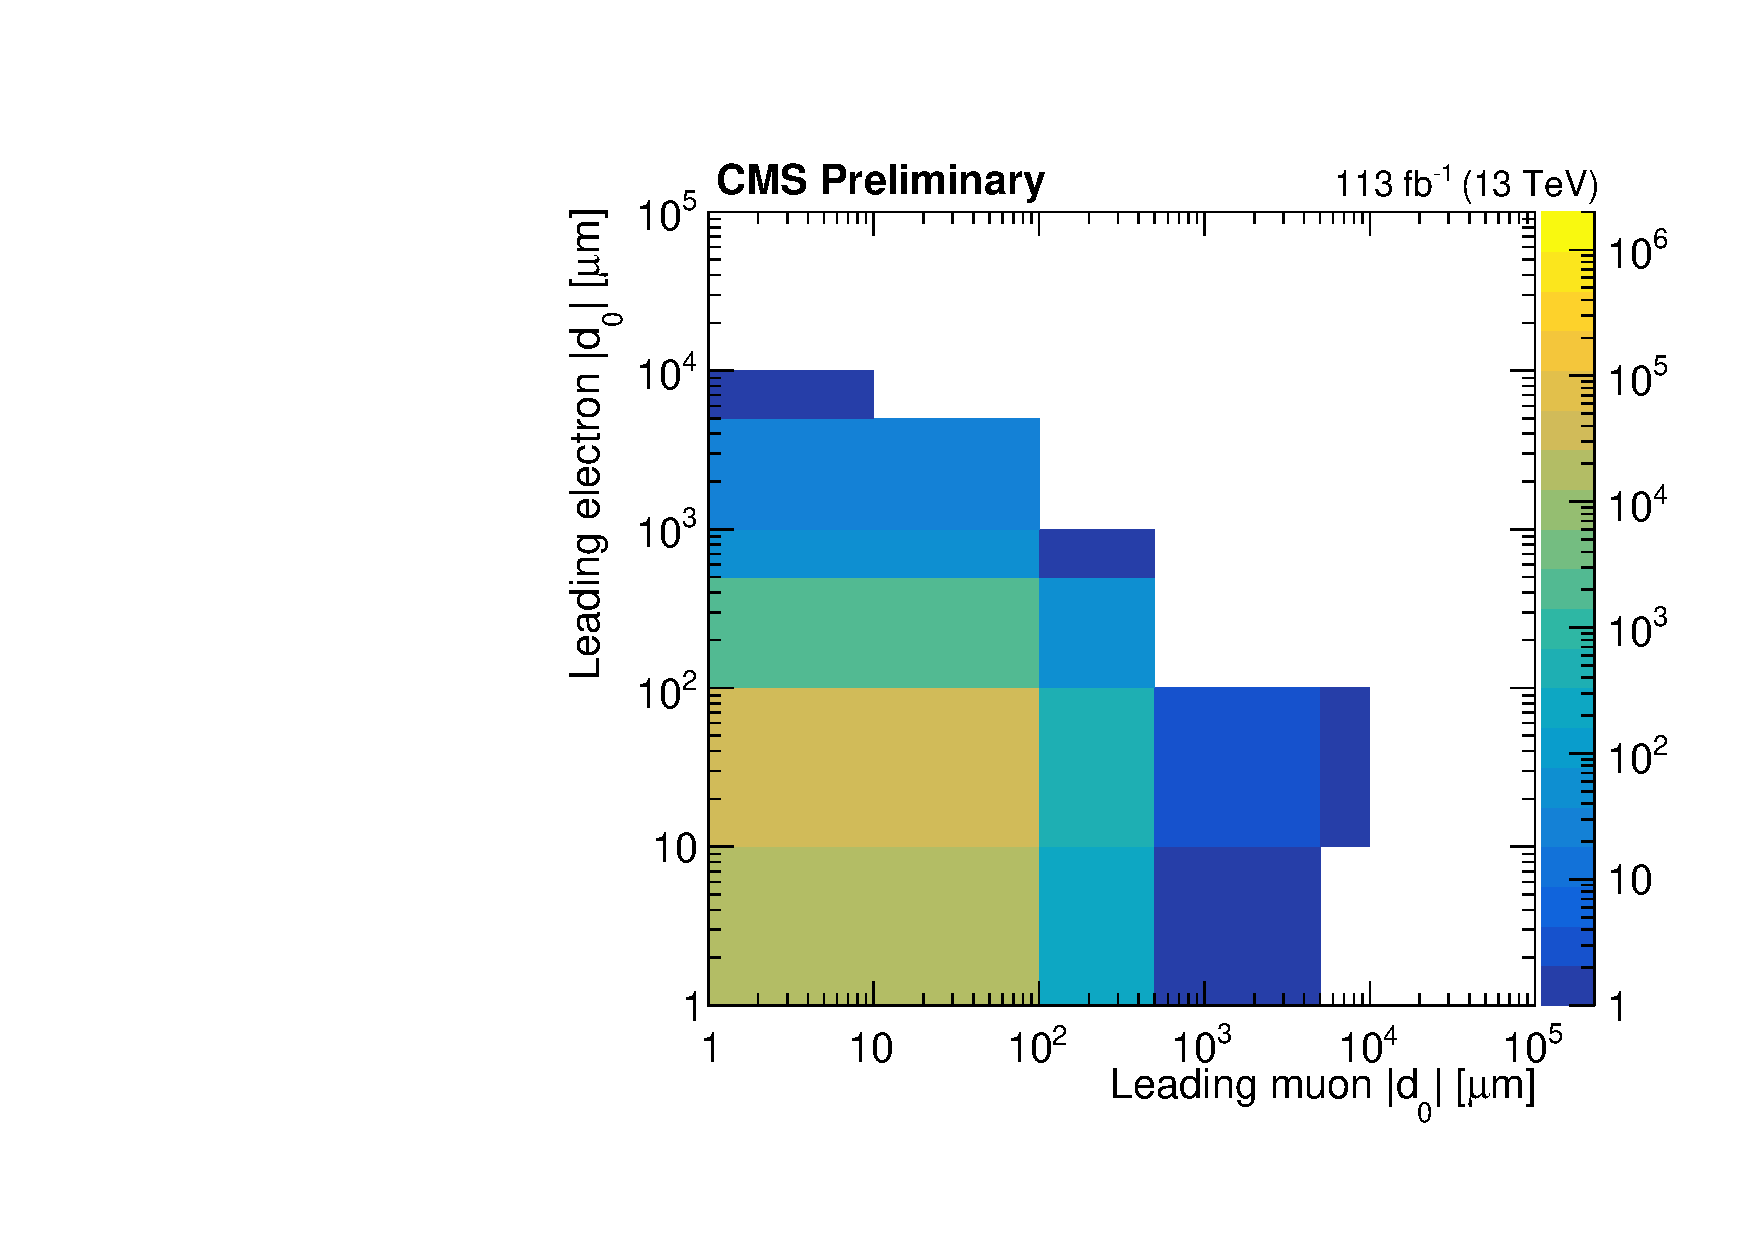
\includegraphics[width=0.32\textwidth]{figures/results/d0vsd0_emu_CMSPreliminary.pdf}
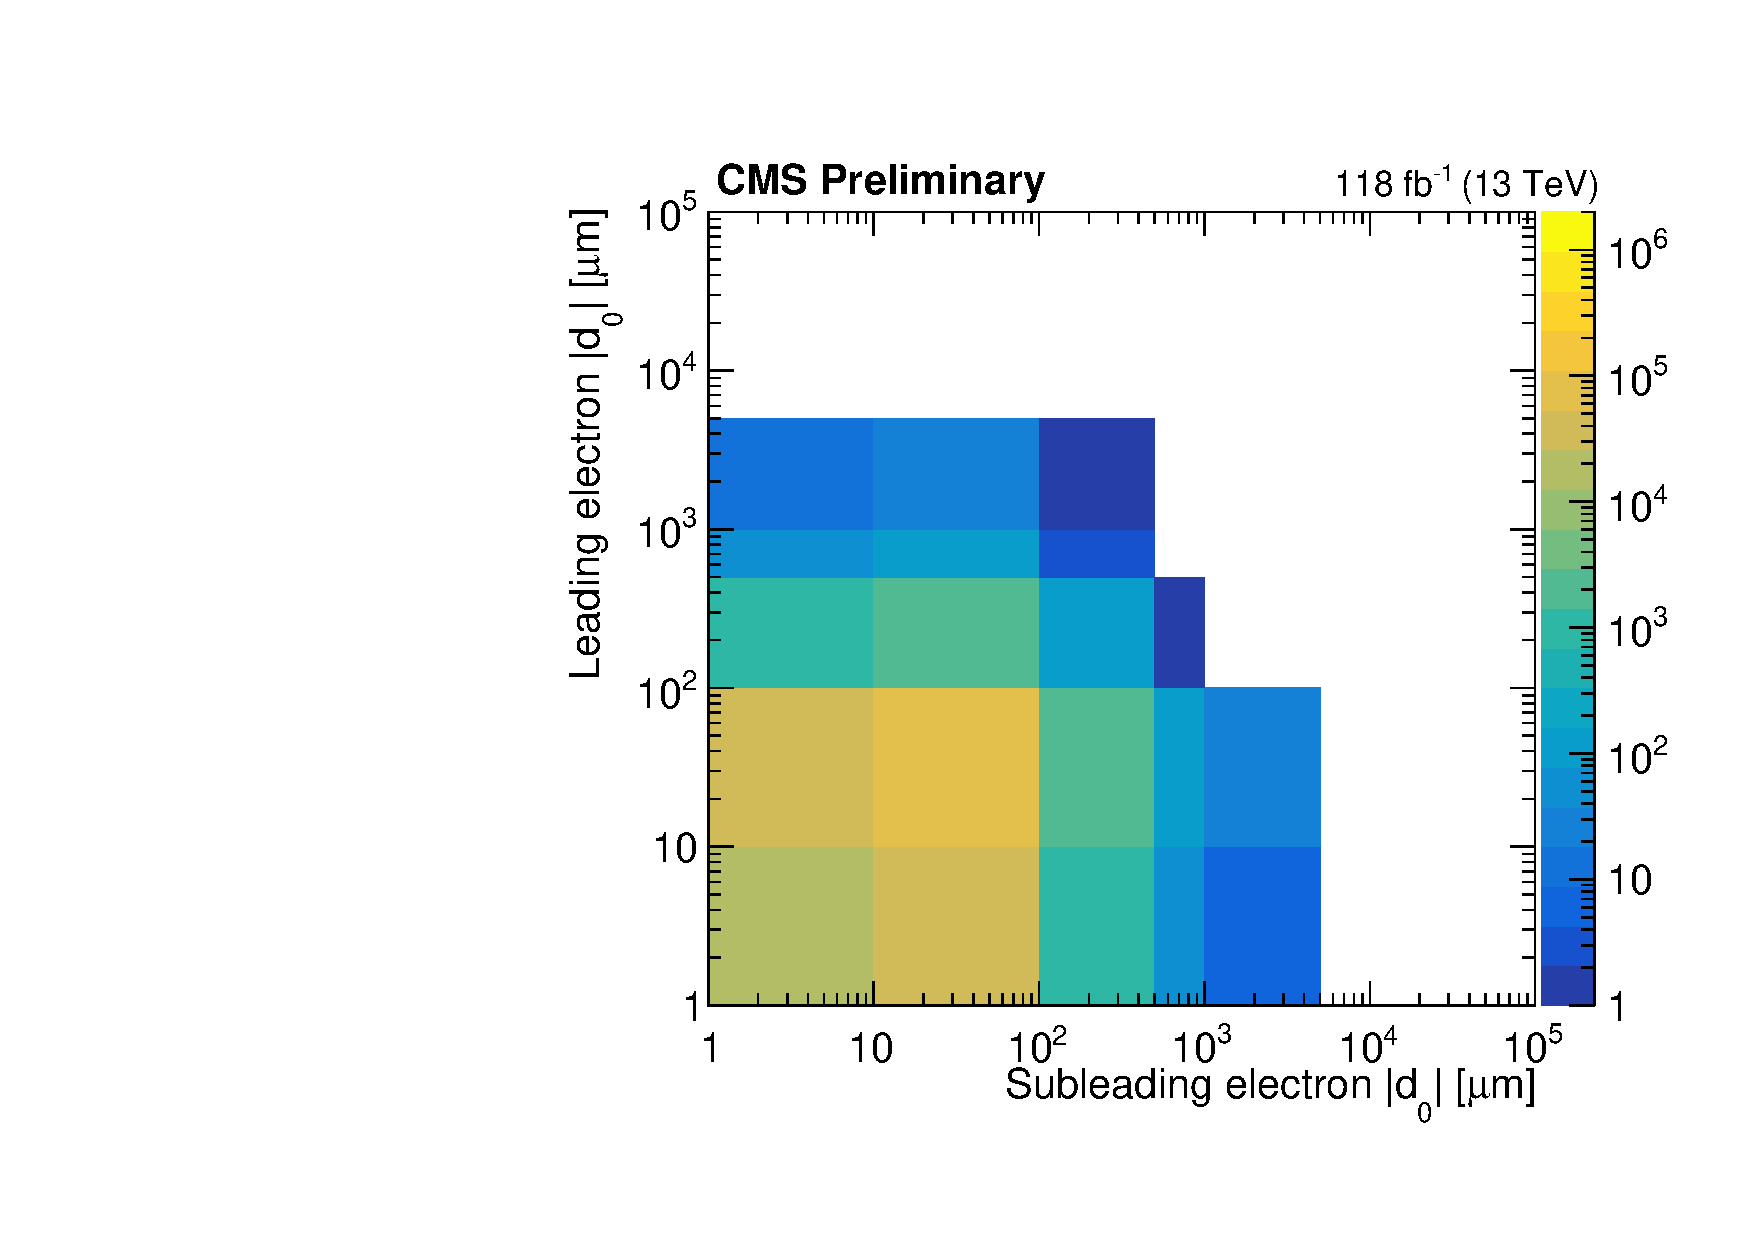
\includegraphics[width=0.32\textwidth]{figures/results/d0vsd0_ee_CMSPreliminary.pdf}
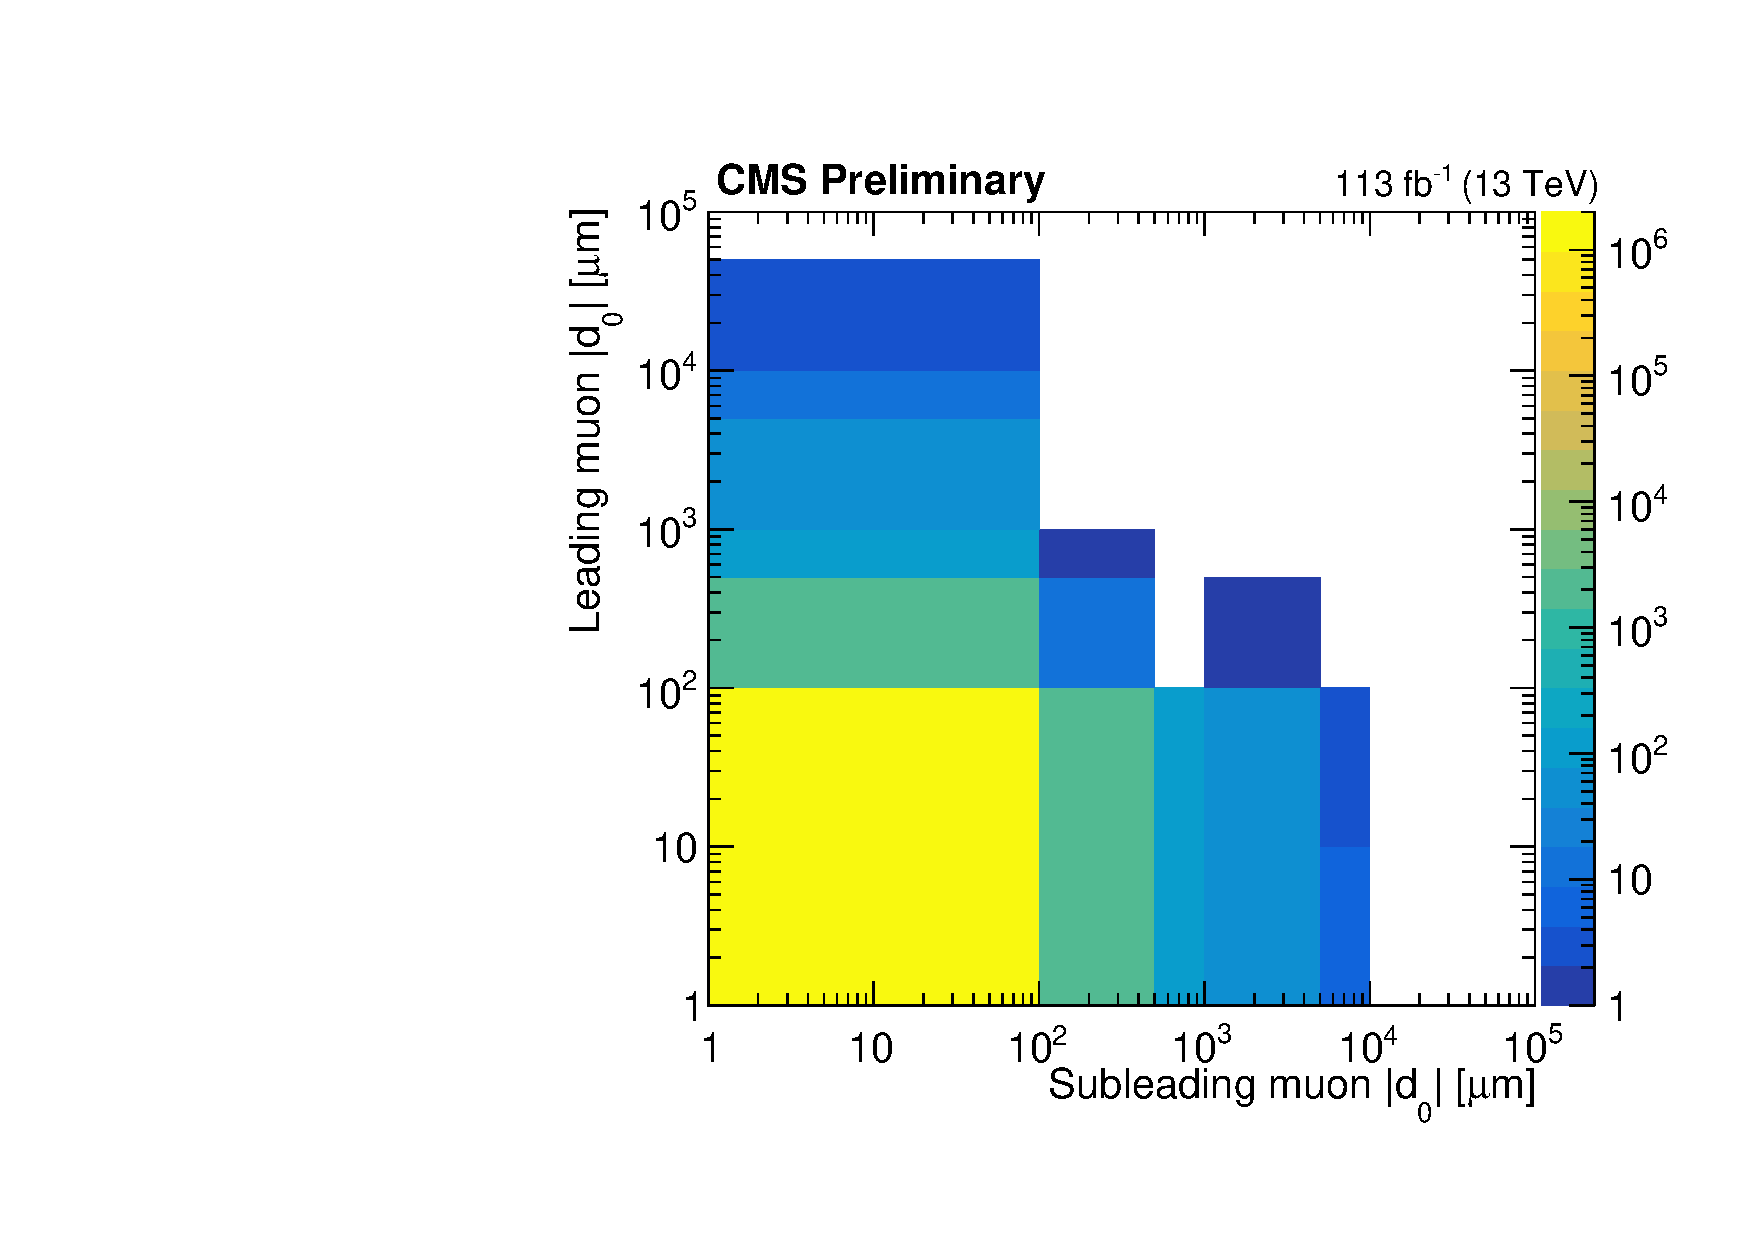
\includegraphics[width=0.32\textwidth]{figures/results/d0vsd0_mumu_CMSPreliminary.pdf}
\caption{
Two-dimensional distributions of \ada and \adb, for the events in data that pass the $\Pe\Pgm$ (left), $\Pe\Pe$ (center), and $\Pgm\Pgm$ (right) preselection. The bins along the x and y axes contain underflow. The inclusive signal region covers the region between \SI{100}{\um} and \SI{10}{\cm} in each \ad variable shown.
}
\label{d0_d0_data}
\end{figure}

\begin{figure}
\centering
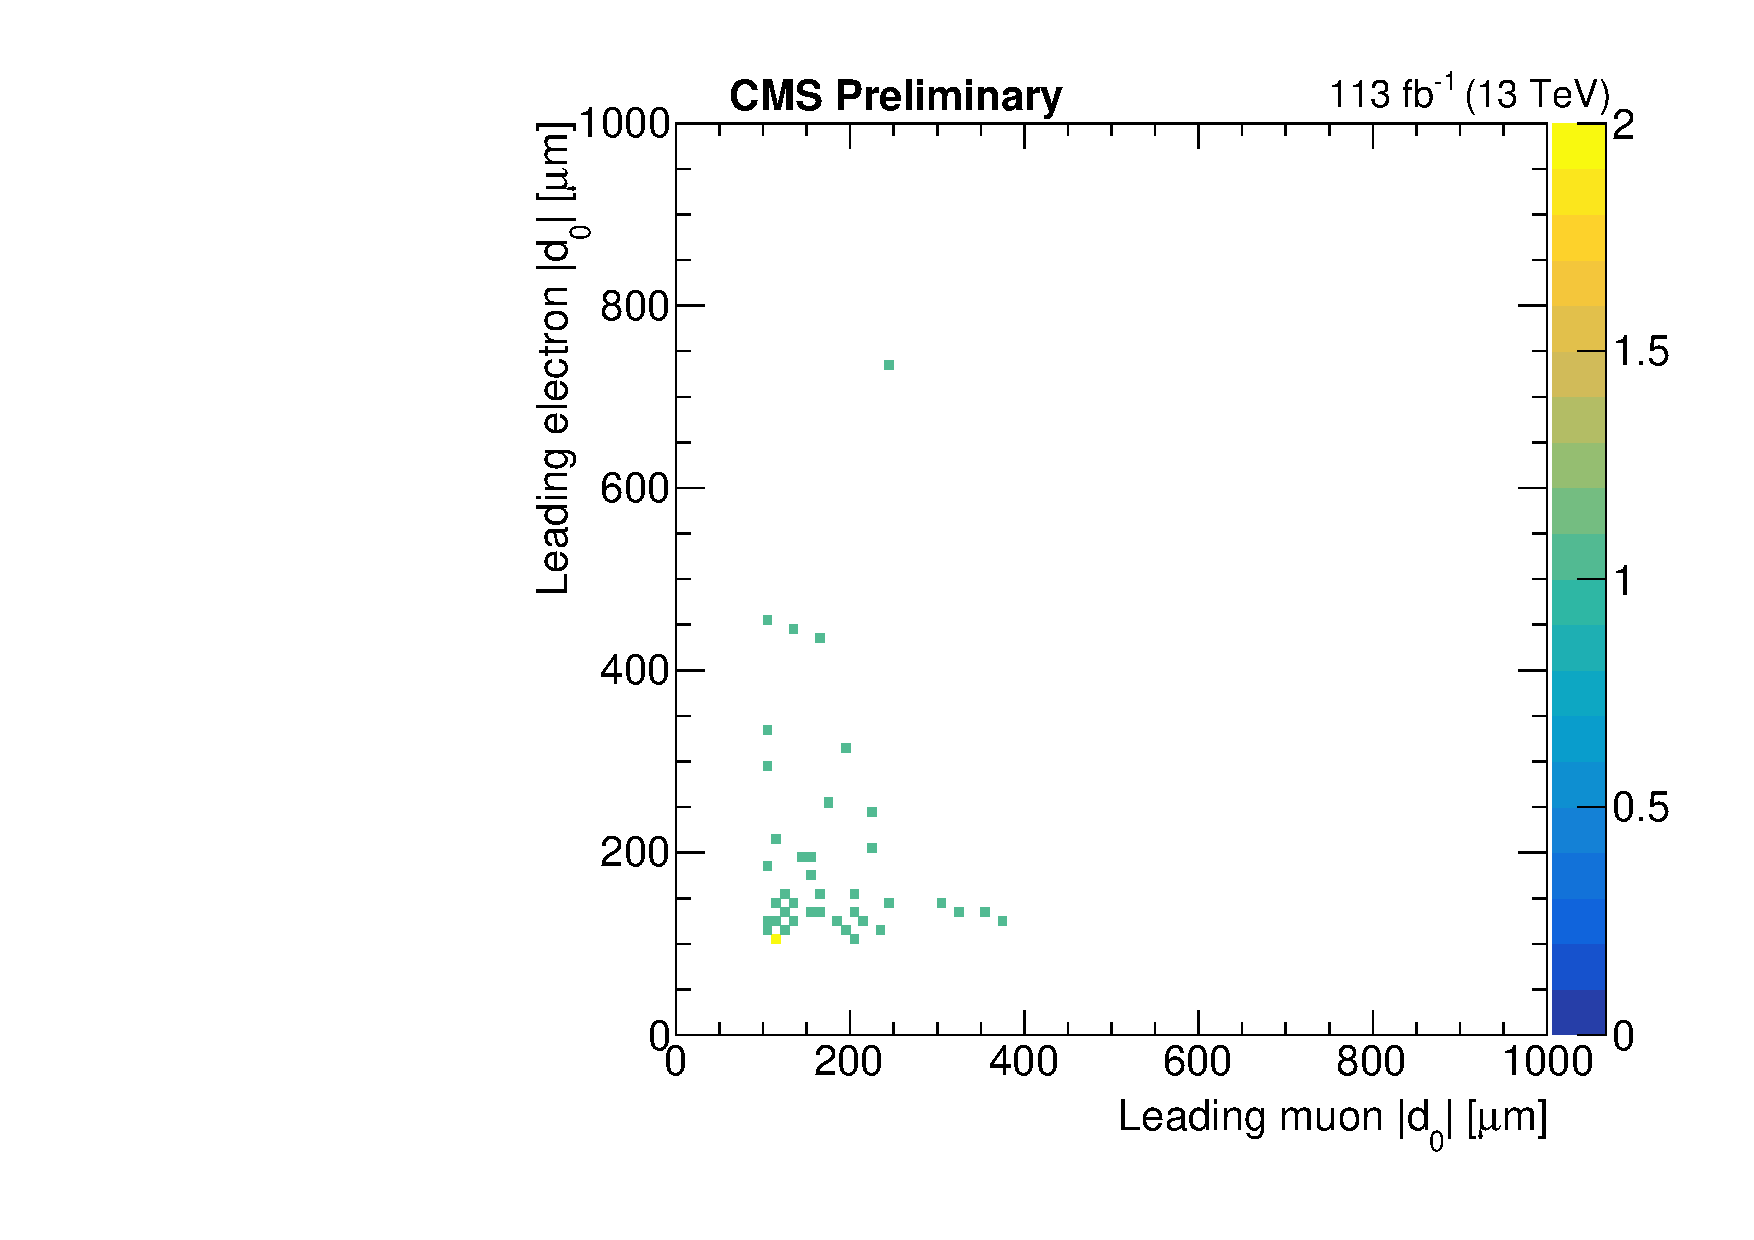
\includegraphics[width=0.31\textwidth]{figures/results/electronAbsD0[0]_vs_muonAbsD0[0]_1000um.pdf}
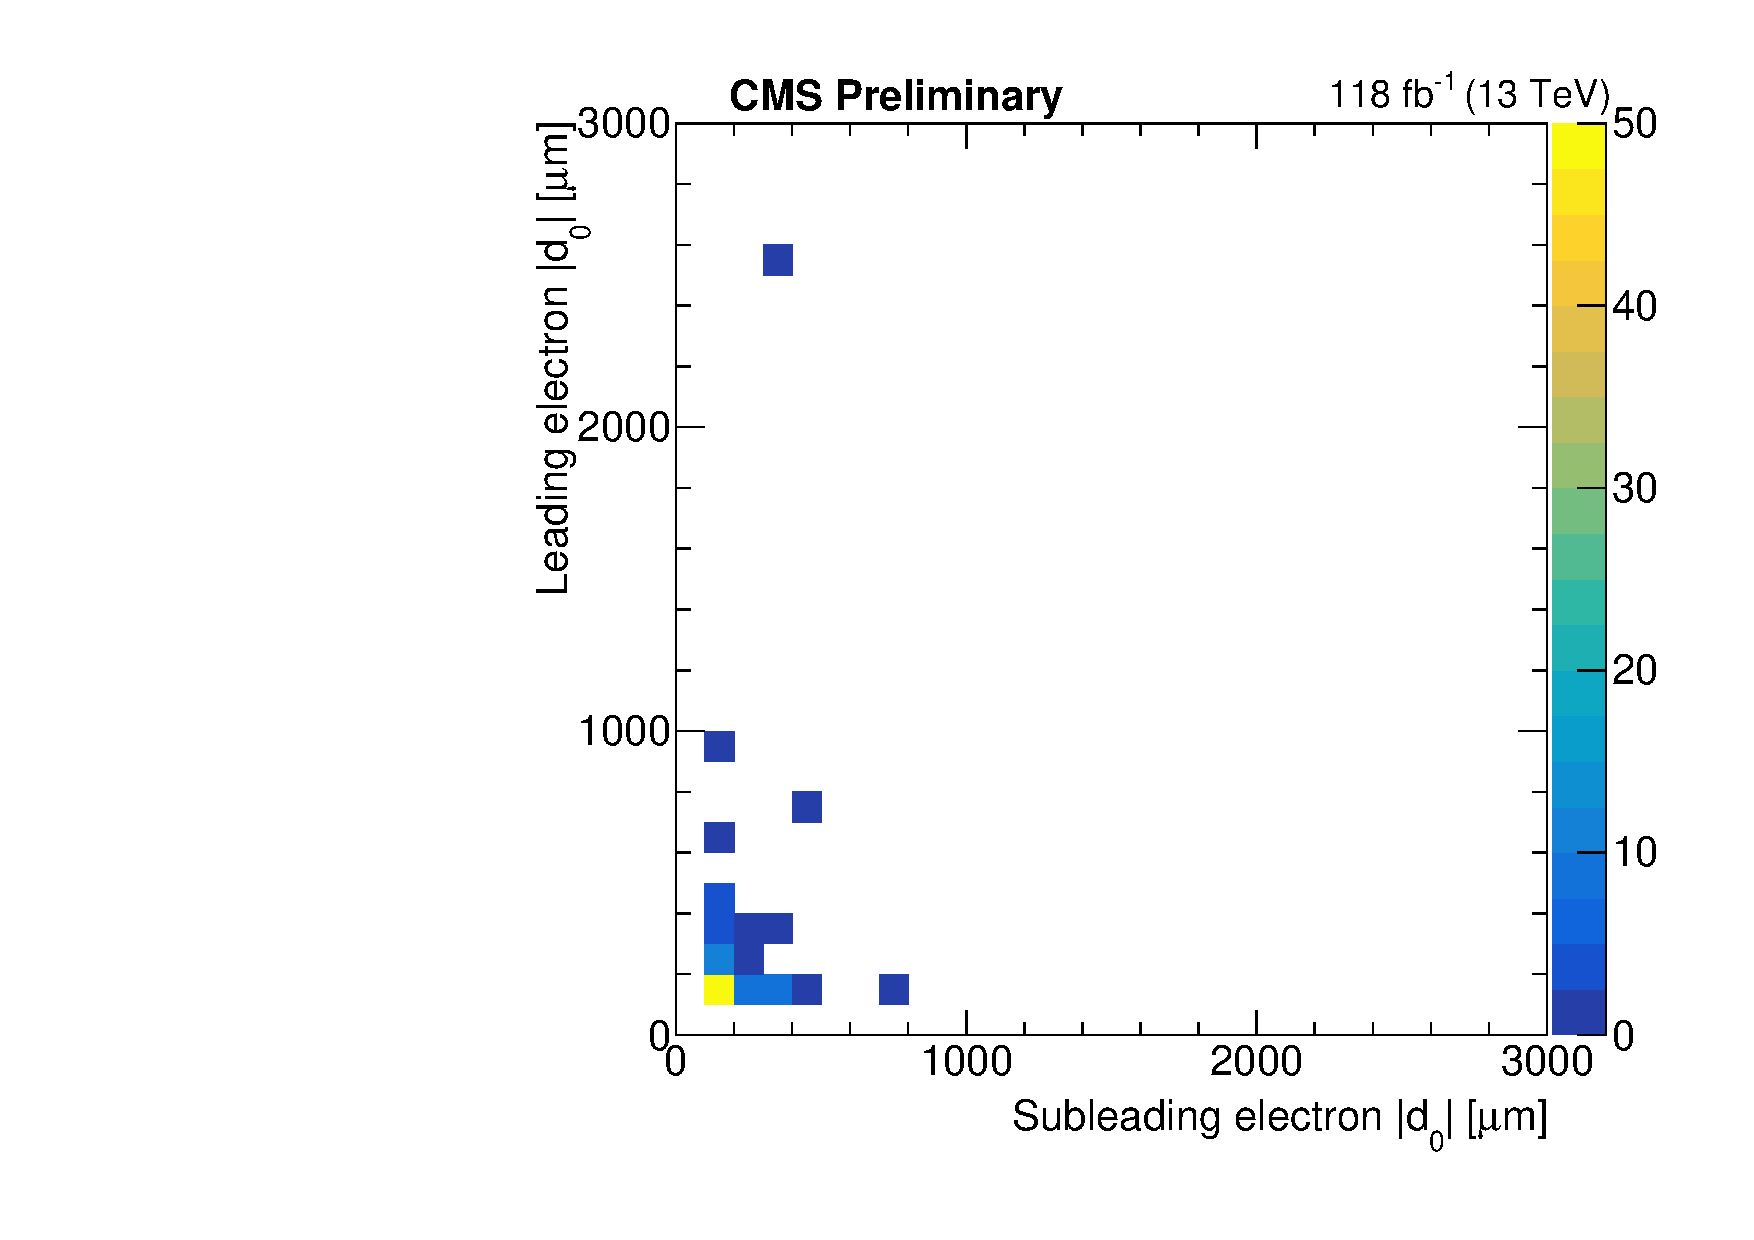
\includegraphics[width=0.31\textwidth]{figures/results/electronAbsD0[0]_vs_electronAbsD0[1]_10000um.pdf}
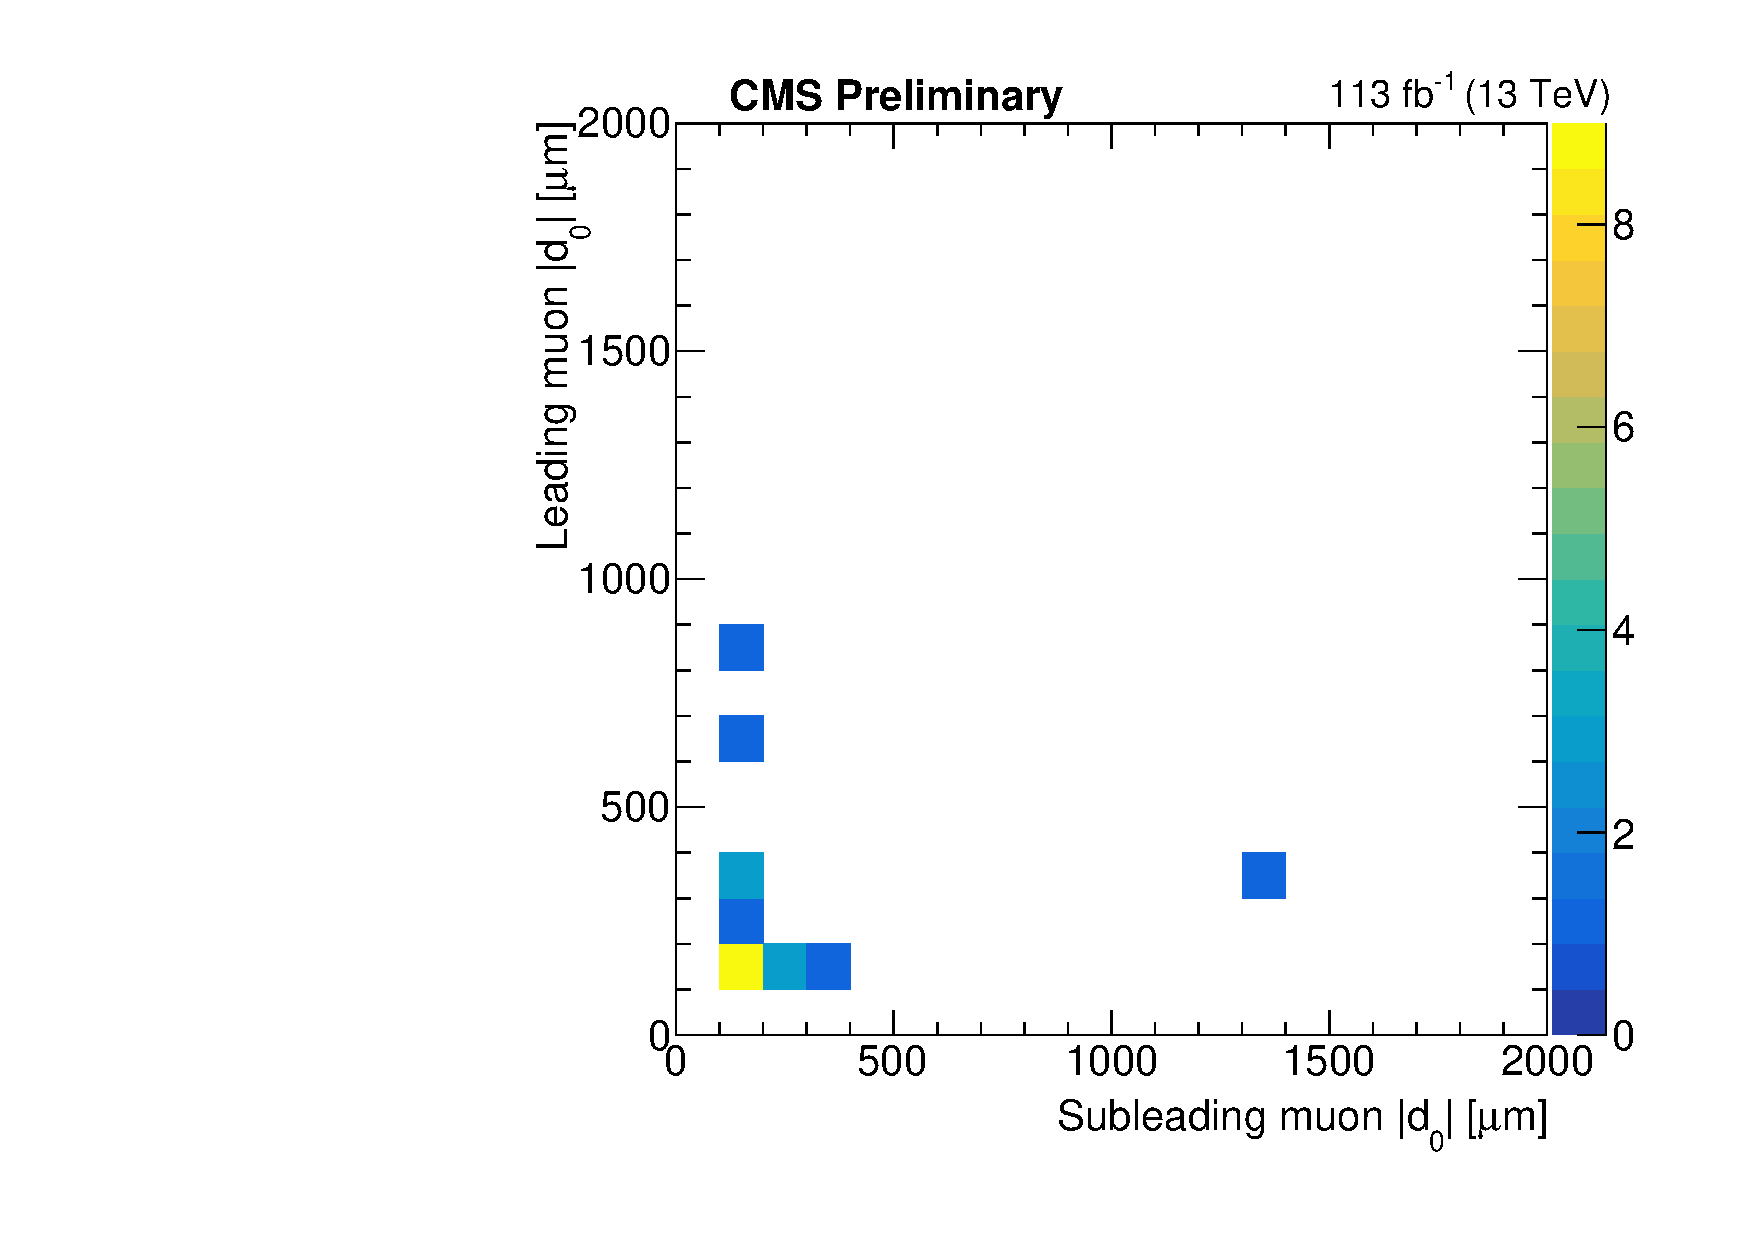
\includegraphics[width=0.31\textwidth]{figures/results/muonAbsD0[0]_vs_muonAbsD0[1]_10000um.pdf}
\caption{
Two-dimensional distributions of \ada and \adb, for data events in the inclusive SR in the $\Pe\Pgm$ (left), $\Pe\Pe$ (center), and $\Pgm\Pgm$ (right) channels.
}
\label{d0_d0_sr_data}
\end{figure}